\documentclass[german, 12pt]{book}
%\usepackage{url}
\PassOptionsToPackage{hyphens}{url}\usepackage[breaklinks=true]{hyperref}
\usepackage{dsfont}
\usepackage{listings}
\usepackage{german}
\usepackage[utf8]{inputenc}
\usepackage[final]{graphicx}
\usepackage{float}
\usepackage{geometry}
\usepackage{setspace}

\geometry{a4paper, top=30mm, left=30mm, right=20mm, bottom=35mm, headsep=10mm, footskip=12mm}


\begin{document}
	
\onehalfspacing

\title{SharkNet\\
Systembeschreibung \\
Version 0.0.3
}

\author{
Dustin Feurich
}

\maketitle

\tableofcontents

\chapter{Überblick}



\subsection{Einleitung}
Durch die rasante Entwicklung des Internet of Things (IoT) ist das Interesse an einen semantischen Datenaustausch spürbar gestiegen. Wurde in den letzten Jahrzehnten noch fast ausschließlich klassisch über die Zieladresse der Datenpakete geroutet, so werden jetzt auch die Metadaten dieser Datenpakete beim Routing zunehmend beachtet. Das Routing erfolgt hierbei inhaltsbasiert und ermöglicht ein Routing nach den Interessen der Kommunikationsteilnehmer. Der Datenaustausch zwischen diesen Teilnehmern kann beim inhaltsbasierten Routing sowohl per klassischer Client-Server Architektur, als auch über Peer-To-Peer (P2P) erfolgen. In dieser Arbeit wird der Datenaustausch über P2P erfolgen, was mehrere Vorteile bietet:
\begin{itemize}
\item Die Verbindungen zwischen Kommunikationsteilnehmern (Peers) können spontan aufgebaut werden, es wird keine Serverinfrastruktur benötigt.
\item Die Daten liegen ausschließlich bei den Peers selbst. Da es keine Zwischenstation für die Datenpakete gibt, erhöht dies die Vertraulichkeit der Kommunikation immens. 
\item Nahezu alle Kommunkationsanwendungen verwenden das Internet um den Datenaustausch zu ermöglichen. Eine Verbindung mit dem Internet ist jedoch nicht zu jeder Zeit und an jedem Ort verfügbar. Weiterhin kann auch hier auf den Zwischenservern die Kommunikation gespeichert und an Dritte weitergegeben werden.
\end{itemize}  
Der dezentrale Austausch von Daten wird unter anderem in der Android-Anwendung SharkNet realisiert. Die App verwirklicht ein dezentrales soziales Netzwerk, bei dem alle Daten ausschließlich innerhalb der Geräte gespeichert sind, es gibt keinen mithörenden zentralen Server. \\Ziel des neuen Protokolls soll es sein, dass die Benutzer der App Nachrichten an andere sich in der Nähe befindenden Benutzer versenden können. Das Routing dieser Nachrichten soll inhaltsbasiert ablaufen, so dass allein die semantische Beschreibung des Nachrichteninhalts und das Interesse der Benutzer die Route vorgibt. SharkNet hat im Kommunikationsbereich dafür einige bereits lauffähige Komponenten, für die Umsetzung des geplanten Protokolls sind aber neben der Anpassung von Alten auch neue Komponenten erforderlich. 
\newline [...]
\newpage
\subsection{Struktur}
Die Arbeit hat überwiegend einen für Informatik-Abschlussarbeiten klassischen Aufbau. Nach einer kurzen Einleitung werden die benötigten Grundlagen erläutert und anschließend wissenschaftliche Paper vorgestellt, die ein ähnliches Thema haben. Das Kapitel Entwurf erklärt den Aufbau und den Geltungsbereich des Protokolls sowie die Architektur und Oberfläche der App. Das Kapitel Implementierung beinhaltet die Komponenten, die für diese Arbeit weiterentwickelt und gänzlich neu entworfen worden sind. Die Beschreibung einer Komponente erfolgt dabei immer nach folgendem Schema:
\begin{enumerate}
	\item Es wird zunächst die Aufgabe und Bedeutung der Komponente innerhalb der App dargestellt.
	\item Anschließend wird die Architektur der Komponente mit Abbildungen vorgestellt.
	\item Darauf folgen die Hinweise, inwiefern die Komponente durch andere Softwareentwickler genutzt werden kann.
	\item Für jede Komponente gibt es außerdem ein eigenes Kapitel zum Thema Test, dies umfasst je nach Komponentenart verschiedene Testarten
	\item Abgeschlossen wird die Beschreibung der Komponente durch einen Ausblick, in dem festgehalten wird, auf welche Art und Weise die Komponente in Zukunft noch verbessert werden könnte.
\end{enumerate}
In dem sich anschließenden Kapitel Test wird ausschließlich die gesamte Anwendung getestet, die spezifischen Tests befinden sich in den Komponentenbeschreibungen. 
\newline Abgerundet wird die Arbeit durch ein abschließendes Fazit und einen Ausblick, der die Chancen und Erweiterungsmöglichkeiten der Anwendung zum Inhalt hat.
\newpage




\chapter{Bluetooth}


\subsubsection{Aufgabe der Komponente}
Die über SharkNet abgeschickten Nachrichten werden über Bluetooth übertragen. Die Komponente ist dabei ausschließlich für die kabellose Übertragung von Daten bzw. Nachrichten verantwortlich, die Ortung von potentiellen Kommunikationspartern erfolgt über die Wifi-Direct Komponente. Auch die Filterung von bereits bekannten oder semantisch uninteressanten Nachrichten wird nicht innerhalb dieser Komponente, sondern innerhalb der Semantischen Routing Komponente vorgenommen.
\\Da es in SharkNet neben normalen Chats auch Gruppenchats und einen semantischen Broadcast gibt, erfordert der Datenaustausch mit Bluetooth kein Pairing der miteinander kommunizierenden Geräte. Dies trägt maßgeblich zur Benutzerfreundlichkeit bei, da insbesondere beim semantischen Broadcast sonst ständig Anfragen zum Pairing auf dem Gerät erscheinen würden und vom Benutzer zusätzliche Interaktionen erforderlich wären.



\subsubsection{Architektur}

\subsubsubsection{Überlick}\label{ch:bluetoothoverview}

Im folgenden UML-Klassendiagramm sind alle Bestandteile der Bluetooth Komponente von SharkNet abgebildet.
\begin{figure}[H]
	\centering
	\hspace*{1cm}
	\makebox[\linewidth][c]{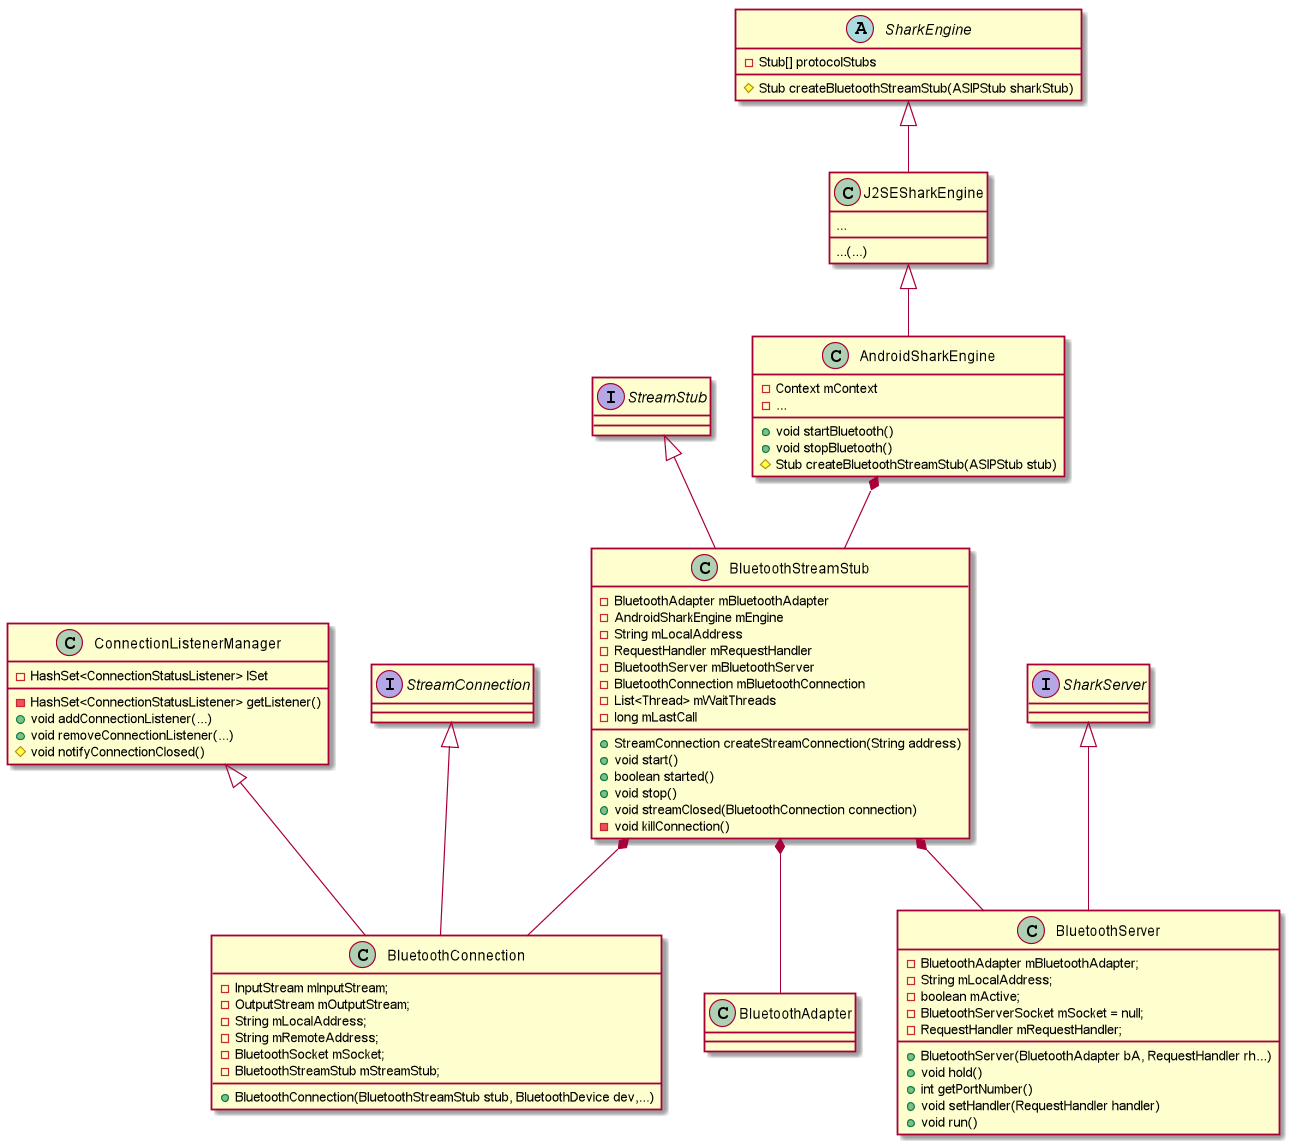
\includegraphics[width=1.1\linewidth]{bluetooth/images/bluetoothGesamt.png}}%
	\caption{Die Bluetooth Klassen im Überblick}
	\label{fig:bluetoothAll}
\end{figure}
Im Zentrum dieser Hierarchie steht die Klasse \textit{BluetoothStreamStub}. Eine Instanz dieser Klasse befindet sich als Attribut in der Klasse \textit{AndroidSharkEngine}, von der aus alle Protokolle wie NFC, Wifi-Direct oder Bluetooth gesteuert werden. Sie stellt daher auch Methoden wie \textit{startBluetooth()} oder \textit{stopBluetooth()} bereit. 





\subsubsubsection{Schnittstellendefinitionen}\label{ch:bluetoothinterfaces}
Anhand der Klassenhierarchie der Bluetooth-Komponente lässt sich erkennen, dass die folgenden drei Schnittstellen implementiert werden:
\begin{itemize}
	\item \textit{StreamStub}: Mit Hilfe von Implementierungen dieses Interfaces können streambasierte Ende-zu-Ende Verbindungen zwischen zwei Geräten hergestellt werden. Die Klasse BluetoothStreamStub öffnet und schließt daher die Verbindungen zu anderen Geräten per Bluetooth.
	\item \textit{StreamConnection}: Das Shark Framework definiert mit dem Interface StreamConnection das Verhalten einer streambasierten Verbindung zweier Geräte. Dieses Interface ist nicht zu verwechseln mit gleichnamigen Interface von Java ME. Klassen wie \textit{BluetoothConnection}, welche dieses Interface implementieren, bauen in ihren jeweiligen Konstruktur die Verbindung mit ihrem jeweiligen Protokoll auf. In der Klasse \textit{BluetoothConnection} erfolgt dies über das Bluetooth-Protokoll RFCOMM.
	\item \textit{SharkServer}: Eine dieses Interface implementierende Klassen wartet bei der bestehenden Verbindung auf Datenpakete, nimmt diese an und leitet sie an einen \textit{Request Handler} weiter. Die Klasse \textit{BluetoothServer} nimmt daher die Datenpakete an, die per bestehender Bluetoothverbindung eintreffen.

\end{itemize}

\subsubsection{Nutzung}
Der Start der Komponente erfolgt automatisch mit dem Start der Anwendung durch eine Instanzierung der Klasse \textit{AndroidSharkEngine}. Sie kann jedoch in ebenjener Klasse durch die Methoden \textit{startBluetooth()} und \textit{stopBluetooth()} auch manuell gestartet sowie gestoppt werden.

\subsubsubsection{Code}
Der Code dieser Komponente kann hier \url{https://github.com/SharedKnowledge/SharkNet-Api-Android/tree/master/api/src/main/java/net/sharksystem/api/shark/protocols/bluetooth} betrachtet werden. Wie auch die anderen Implementierungen von Über\-tra\-gungs\-pro\-to\-kol\-len, befindet sich auch die Bluetooth-Implementierung im Projekt \textit{SharkNet-Api-Android} im Package \textit{protocols}. 
\\Es werden nun die wichtigsten Codezeilen der drei im Unterkapitel Schnittstellendefinitionen erwähnten Klassen beschrieben.
\\Der \textit{BluetoothServer} horcht auf eingehende Verbindungen mit Hilfe der von Android bereitgestellten Klasse \textit{BluetoothSocket}, die folgendermaßen initialisiert wird:
 \lstset{language=Java, caption=Initialisierung des Bluetooth-Server-Sockets, label=DescriptiveLabel, numbers=left, numbersep=1em, breaklines=true, basicstyle=\small}
\begin{lstlisting}
mSocket = mBluetoothAdapter.listenUsingInsecureRfcommWithServiceRecord(BluetoothStreamStub.BT_NAME, BluetoothStreamStub.BT_UUID);
\end{lstlisting}
Hierbei wird mit Hilfe des aktiven \textit{BluetoothAdapter}, welcher auch in der Klasse \textit{BluetoothConnection} benutzt wird, über das Bluetooth-Protokoll \textit{RFCOMM} der Server-Socket erzeugt, zu dem sich andere Geräte verbinden können. Es wird statt der sonst gängigen Methode \textit{listenUsingRfcommWithServiceRecord()} die \textit{insecure} Variante genutzt, um kein Bluetooth-Pairing zwischen den Geräten vorher durchführen zu müssen. Der nächste Auszug zeigt die Annahme von eingehenden Verbindungen auf Serverseite:
 \lstset{language=Java, caption=Serverseitige Annahme der Bluetooth-Verbindungen (Auszug), label=DescriptiveLabel, numbers=left, numbersep=1em, breaklines=true, basicstyle=\small}
\begin{lstlisting}
try {
  while (mActive){
    BluetoothSocket bluetoothSocket = mSocket.accept();
    BluetoothConnection con = new BluetoothConnection(bluetoothSocket, mLocalAddress);
    mRequestHandler.handleStream(con);
  }
  mSocket.close();
\end{lstlisting}
Die Annahme der Anfrage geschieht in der dritten Zeile, wobei der daraus resultierende \textit{BluetoothSocket} in der folgenden Zeile für den Aufbau einer Verbindung genutzt wird. Die Verbindung wird anschließend vom Shark-Interface \textit{RequestHandler} verwertet. Dies bedeutet, dass die im Stream enthaltene Nachricht innerhalb der Framework-Ebene nun weiterverarbeitet wird. Dies schließt unter anderem auch die semantische Auswertung der Nachricht mit ein.
\\Der Aufbau einer Bluetooth-Verbindung erfolgt auf Clientseite ähnlich zum Aufbau auf der Serverseite innerhalb der Klasse \textit{BluetoothConnection}:
 \lstset{language=Java, caption=Clientseitige Initialisierung des Sockets, label=DescriptiveLabel, numbers=left, numbersep=1em, breaklines=true, basicstyle=\small}
\begin{lstlisting}
mSocket = device.createInsecureRfcommSocketToServiceRecord(BluetoothStreamStub.BT_UUID)
\end{lstlisting}
Auch hier wird die \textit{Insecure} Variante der Methode genommen, um auf ein Pairing verzichten zu können.
\\Instanzen der beiden bisher vorgestellten Klassen \textit{BluetoothServer} und \textit{BluetoothStreamStub} werden durch die Klasse \textit{BluetoothStreamStub} erzeugt und verwaltet. Neben der Erzeugung dieser Objekte liefert der \textit{BluetoothStreamStub} weiterhin die lokale Bluetooth MAC-Adresse des Geräts:
\textit{BluetoothConnection}:
\lstset{language=Java, caption=Auslesen der Bluetooth MAC-Adresse, label=DescriptiveLabel, numbers=left, numbersep=1em, breaklines=true, basicstyle=\small}
\begin{lstlisting}
mLocalAddress = android.provider.Settings.Secure.getString(engine.getContext().getContentResolver(), "bluetooth_address");
//mLocalAddress = BluetoothAdapter.getDefaultAdapter().getAddress() Nur vor Marshmallow nutzbar, liefert nach dieser Version nur eine unbrauchbare Konstante!
\end{lstlisting}
Dies geschieht zwangsweise über eine Reflektion, da die bis Android-Marshmallow dafür vorhergesehene Methode nur eine Konstante liefert, die nicht der eigentlichen Bluetooth MAC-Adresse des Geräts entspricht. Die Bluetooth MAC-Adresse wird jedoch zwingend für \textit{Insecure} Verbindungen benötigt, welche kein Bluetooth-Pairing erfordern, was für die Broadcast-Komponente essentiell ist. 
\\Die restlichen Methoden der Bluetooth-Komponente wie beispielsweise \textit{killConnection()} sind mnemonischer Natur.

\subsubsubsection{Deployment / Runtime}
\newline [...]


\subsubsection{Test}
\subsubsubsection{Gerätetest}
Mit den folgenden Android-Geräten ist die Komponente auf Kompatibilität geprüft worden:
\begin{table}[H]
	\begin{center}
		\caption{Kompatibilitätstest der Bluetooth-Komponente}
		\label{tab:dimensions}
		\begin{tabular}{l|c|c} 			
			Gerät & Android-Version & kompatibel \\
			\hline
			LG Nexus 5x & 8.0 & Ja\\
			LG Nexus 5x & 8.1 & Nein\\
			LG Nexus 5 & 6.1 & Ja\\
			Sony Xperia XZ Premium & 8.0 & Ja\\
			Sony Xperia Z4 Tablet & 7.1.1 & Ja\\
			Lenovo B & 6.0 & Ja\\
			Lenovo A5500-F Tablet & 4.4 & Nein\\
			Raspberry Pi 3 & 6.0.1 & Ja\\	
			Wandboard Quad & 5.0.2 & Ja\\			
		\end{tabular}
	\end{center}
\end{table}
Seit neusten Android-Version 8.1 ist es nicht mehr mit der in Listing 4.4 beschriebenen Refeklektion möglich, die Bluetooth MAC-Adresse programmatisch auszulesen. Dementsprechend kann das Testgerät Nexus 5x seit dem Update des Betriebssystems keine Nachrichten via Bluetooth mehr empfangen, da die anderen Geräte keine valide MAC-Adresse vom Nexus 5x erhalten haben und die Verbindung somit ohne Pairing nicht erfolgreich aufgebaut werden kann. 
\\Beim Lenovo A5500-F Tablet handelt es sich um eine zu alte Android-Version, wodurch in mehreren Komponenten zu Exceptions kommt, weil benötigte Methoden noch nicht enthalten sind.



\subsubsection{Ausblick}
Es ist empfehlenswert, die von Android gestellten Bluetooth Klassen durch die dazu äquivalenten Bluetooth Low Energy (BLE) Klassen entweder zu ersetzen oder zumindest eine Alternative zu dem klassischen Bluetooth Package zu bieten. BLE verbraucht weit weniger Akkuleistung als das klassische Bluetooth, kann dafür aber nur eine geringere Menge an Daten pro Verbindung unterstützen. Da die mit SharkNet verschickten Nachrichten auch trotz der semantischen Annotationen nur wenige Kilobyte benötigen, stellt dies für SharkNet kein Hindernis dar.
\\Notwendig ist zukünftig außerdem das Ersetzen der in Listing 4.4 dargestellten Reflektion zum Auslesen der Bluetooth MAC-Adresse. Dies funktioniert nur mit Geräten bis einschließlich Android 8.0, ab Android 8.1 ist die ausgelesene MAC-Adresse inkorrekt. Über die WiFi-Komponente an andere Geräte versendete inkorrekte Bluetooth-Adressen führen dann dazu, dass das Gerät keine Nachrichten über Bluetooth empfangen kann. 
\\Lasttests mit mehreren miteinander kommunizierenden Geräten und gleichzeitigem Spammen von Nachrichten haben der Komponente ebenfalls Grenzen der Belastbarkeit aufgezeigt. So können bei zu hoher Last Nachrichten verloren gehen, da das Empfangsgerät die in Listing 4.2 gezeigte \textit{accept()} Methode nicht aufgerufen wird. 
\newpage



\chapter{WiFi}
\subsubsection{Aufgabe der Komponente}
Über die WiFi-Direct Komponente vermitteln die Peers ihre Kontaktdaten an alle ver\-füg\-ba\-ren Peers in der Nähe. Dies geschieht über den Expose Befehl des ASIP Protokolls, bei dem ein ASIP-Interesse an die Wissensbasis von anderen Peers gesandt wird. Dies beinhaltet unter anderem die Bluetooth MAC-Adresse, mit der dem Peer dann anschließend Nachrichten per Bluetooth geschickt werden können. Das Übermitteln der Bluetooth Mac-Adresse via WiFi-Direct ermöglicht es daher, dass für die darauf folgende Bluetooth-Verbindung kein Pairing benötigt wird. 
\\Die Komponente ist der elementare Bestandteil des Peer-Radars, der alle sich in der Nähe befindlichen Peers anzeigt und die Kommunikation mit diesen erlaubt. Das Radar ist wiederum dafür erforderlich, neue Chats mit Peers anzulegen oder einen semantischen Broadcast ohne Bluetooth-Pairing zu ermöglichen.
\begin{figure}[H]
	\centering
	\makebox[\linewidth][c]{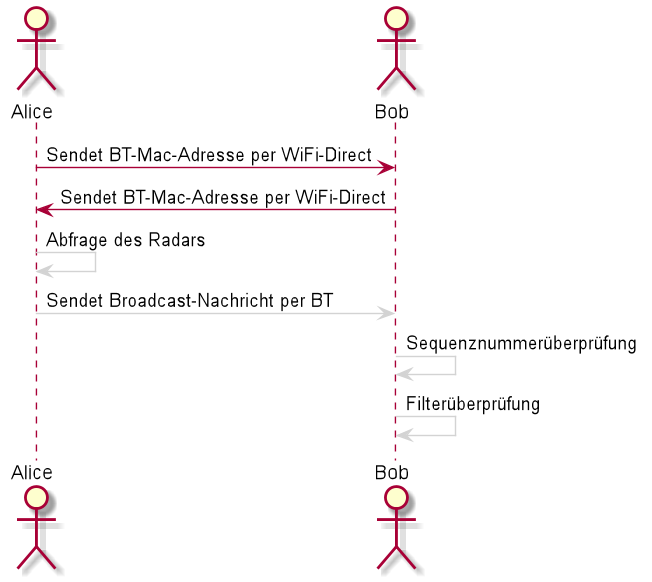
\includegraphics[width=0.6\linewidth]{wifi/images/communicationComps.png}}%
	\caption{Die WiFi Komponente innerhalb des Nachrichtenaustauschs}
	\label{fig:wifiComp}
\end{figure}
\newpage
\subsubsection{Architektur}

Im folgenden UML-Klassendiagramm sind alle Bestandteile der WiFi-Direct Komponente von SharkNet abgebildet.
\begin{figure}[H]
	\centering
	\makebox[\linewidth][c]{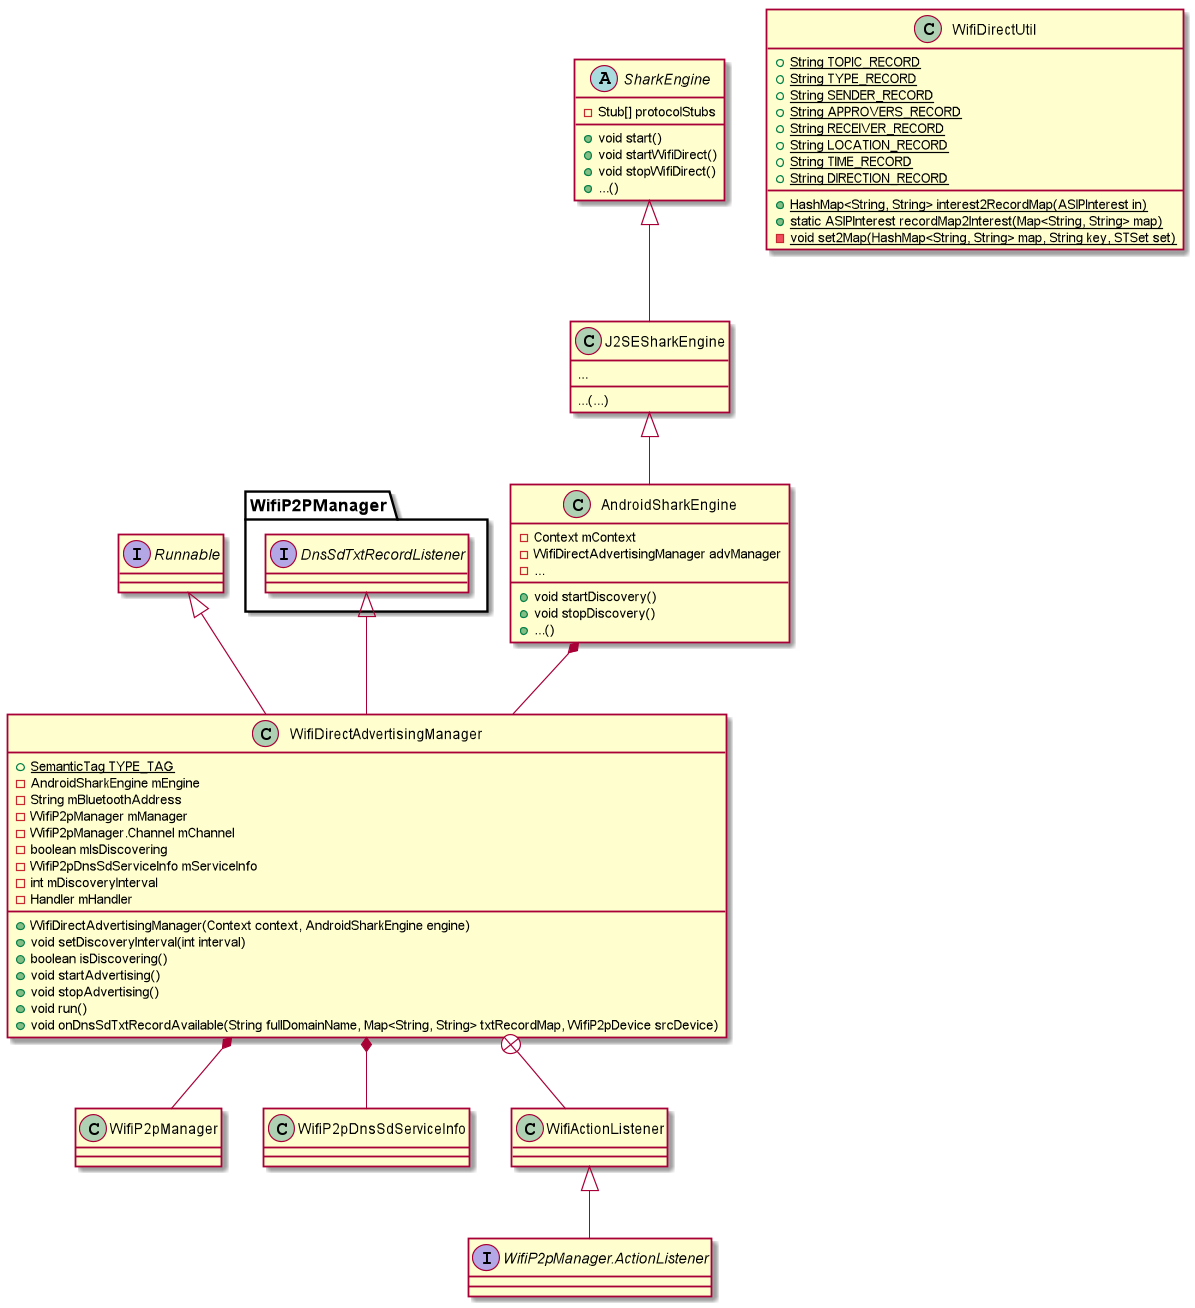
\includegraphics[width=1.1\linewidth]{wifi/images/wifiDirectGesamt.png}}%
	\caption{Die WiFi-Direct Klassen im Überblick}
	\label{fig:wifiAll}
\end{figure}
\newpage
Im Zentrum dieser Hierarchie steht die Klasse \textit{WiFiDirectAdvertisingManager}. Eine Instanz dieser Klasse befindet sich als Attribut in der Klasse \textit{AndroidSharkEngine}, von der aus alle Protokolle wie NFC, Wifi-Direct oder Bluetooth gesteuert werden. Über die Engine kann daher auch das Radar per \textit{startDiscovery()} Methode gestartet oder über die \textit{stopDiscovery()} Methode beendet werden. Das Starten oder Stoppen der kompletten WiFi-Komponente erfolgt dagegen in der Klasse \textit{AndroidSharkEngine}, die den Ausgangspunkt der Vererbungshierarchie darstellt.
\\Die Klasse \textit{WifiDirectUtil} bietet statische Methoden an, mit denen ASIP-Interessen in Hashmaps umgewandelt werden können und umgekehrt. Dies ist notwendig, da die von Android gestellte Basisklasse \textit{WifiP2PManager} bei den Anmeldungen von Services keine ASIP-Interessen, sondern Hashmaps als Parameter akzeptiert.

\subsubsection{Nutzung}
Die WiFi-Komponente wird automatisch beim Start der Anwendung gestartet. Manuell kann die Komponente über die Klasse \textit{AndroidSharkEngine} gesteuert werden, welche wie schon im Überblick erwähnt die beiden Methoden \textit{startDiscovery()} und \textit{stopDiscovery()} enthält.


\subsubsection{Code}
Der Code dieser Komponente kann unter \url{https://github.com/SharedKnowledge/SharkNet-Api-Android/tree/master/api/src/main/java/net/sharksystem/api/shark/protocols/wifidirect} betrachtet werden. Wie auch die anderen Implementierungen von Über\-tra\-gungs\-pro\-to\-kol\-len, befindet sich auch die WiFi-Direct-Implementierung im Projekt \textit{SharkNet-Api-Android} im Package \textit{protocols}.
\\Wie im vorherigen Unterkapitel erläutert, liefern die beiden Methoden \textit{startDiscovery()} und \textit{stopDiscovery()} die Funktionalität, um Peers zu finden und andere Peers über das eigene Interesse in Kenntnis zu setzen. 
\\Bei Aufruf der \textit{startDiscovery()} Methode wird innerhalb der Engine ein neuer \textit{WifiDirectAdvertisingManager} angelegt und anschließend dessen \textit{startAdvertising()} Methode aufgerufen. Innerhalb der \textit{startAdvertising()} Methode wird sich nun auf der dritten Schicht des OSI-Modells begeben, wie der folgende Codeausschnitt zeigt:\newpage
\lstset{language=Java, caption=Hinzufügung des Services, label=DescriptiveLabel, numbers=left, numbersep=1em, breaklines=true, basicstyle=\small}
\begin{lstlisting}
HashMap<String, String> map = WifiDirectUtil.interest2RecordMap(interest);
mServiceInfo = WifiP2pDnsSdServiceInfo.newInstance("_sbc", "_presence._tcp", map);
mManager.addLocalService(mChannel, mServiceInfo, new WifiActionListener("Add LocalService"));
mManager.clearServiceRequests(mChannel, new WifiActionListener("Clear ServiceRequests"));
WifiP2pDnsSdServiceRequest wifiP2pDnsSdServiceRequest = WifiP2pDnsSdServiceRequest.newInstance();
mManager.addServiceRequest(mChannel, wifiP2pDnsSdServiceRequest, new WifiActionListener("Add ServiceRequest"));
\end{lstlisting}
Nachdem in der ersten Zeile eine Hashmap aus dem Interesse erzeugt worden ist, wird diese Hashmap in Zeile zwei als Parameter für die Erzeugung einer Service Information benutzt. Anschließend wird dem \textit{WifiP2PManager} ein neuer lokaler Service hinzugefügt, wobei dieser Service die zuvor erzeugte Service Information enthält. Nachdem etwaige vorherige Service Requests beseitigt worden sind, wird der neue WifiP2P Service Request hinzugefügt. Dadurch wird nun allen Geräte in der Nähe, die auf WifiP2P Verbindungen warten, der WiFi Service Request zur Verfügung gestellt.
\\Neben dem Hinzufügen von Services, müssen diese aber auch empfangen und ausgewertet werden. Dies ist der Grund, warum der \textit{WifiDirectAdvertisingManager} das Interface \textit{Runnable} implementiert. In der dadurch implementierten Methode \textit{run()} werden die von anderen Geräten gesendeten Service Requests empfangen.\newline
\lstset{language=Java, caption=Erkennung von Services, label=DescriptiveLabel, numbers=left, numbersep=1em, breaklines=true, basicstyle=\small}
\begin{lstlisting}
mManager.discoverServices(mChannel, new WifiActionListener("Discover Services"));
mHandler.postDelayed(this, mDiscoveryInterval);
\end{lstlisting}
Sollte ein Service gefunden und erfolgreich eine Peer-To-Peer Verbindung zwischen zwei Geräten aufgebaut werden können, wird nun die aus Listing 1 bekannte Hashmap an das Gerät gesendet, welches den Service gefunden (discovered) hat. Dabei wird automatisch die Methode \textit{onDnsSdTxtRecordAvailable} aufgerufen, welche die empfangene Hashmap in ein ASIP-Interesse umwandelt und dann der Engine weiterreicht.\newline
\lstset{language=Java, caption=Vewertung des Interesses, label=DescriptiveLabel, numbers=left, numbersep=1em, breaklines=true, basicstyle=\small}
\begin{lstlisting}
ASIPInterest interest = WifiDirectUtil.recordMap2Interest(txtRecordMap);
mEngine.handleASIPInterest(interest);
\end{lstlisting}  

\subsubsection{Gerätetest}
Mit den folgenden Android-Geräten ist die Komponente auf Kompatibilität geprüft worden:\\
\begin{table}[H]
	\begin{center}
		\begin{tabular}{l|c|c} 			
			Gerät & Android-Version & kompatibel \\
			\hline
			LG Nexus 5x & 8.0 & Ja\\
			LG Nexus 5x & 8.1 & Ja\\
			LG Nexus 5 & 6.1 & Ja\\
			Sony Xperia XZ Premium & 8.0 & Ja\\
			Sony Xperia Z4 Tablet & 7.1.1 & Ja\\
			Lenovo B & 6.0 & Ja\\
			Lenovo A5500-F Tablet & 4.4 & Nein\\
			Raspberry Pi 3 & 6.0.1 & Nein\\	
			Wandboard Quad & 5.0.2 & Nein\\			
		\end{tabular}
		\caption{Kompatibilitätstest der WiFi-Komponente}
		\label{tab:dimensions}
	\end{center}
\end{table}
Die beiden Einplatinencomputer Raspberry Pi 3 und Wandboard Quad unterstützen zwar grundsätzlich WLAN, jedoch nicht WiFi-Direct. Beim Raspberry Pi 3 wäre WiFi-Direct zwar technisch möglich, benötigt aber zahlreiche Umkonfigurationen, was dadurch dann nicht mehr eine reine Android-Version darstellt. 
\\Das Lenovo A5500-F Tablet hat mit Android 4.4 eine zu alte Version, die nicht alle von der Komponente benötigten WiFi-Direct Klassen bereitstellt. 
\\Nach dem Update des LG Nexus 5x von Android 8.0 auf die Version 8.1 ist zu beachten, dass das Gerät seine Bluetooth MAC-Adresse nicht mehr programmatisch auslesen kann. Dies betrifft vor allem die Bluetooth-Komponente und wird in der dazugehörigen Komponentenbeschreibung vertieft.  

\subsubsection{Ausblick}
Die WiFi Komponente wurde SharkNet hinzugefügt, da der wiederholte Austausch von Kontakdaten zwischen den Geräten mit Bluetooth zu viel Zeit in Anspruch genommen hat. Da jedes Gerät standardmäßig alle zehn Sekunden seine Anmeldedaten an Geräte in der Nähe schickt, musste diese eher ungewöhnliche Aufteilung erfolgen. Wenn zukünftig die Bluetooth-Komponente auf Bluetooth Low Energy umgestellt werden sollte, ist es eventuell möglich, auf die WiFi Komponente zu verzichten und den gesamten Datenaustausch über Bluetooth vorzunehmen. 
\newpage

\chapter{Sonstiges}
In der folgenden Grafik sind alle Bestandteile der WifiDirect Komponente von SharkNet abgebildet.
\begin{figure}[H]
	\centering
	\hspace*{1cm}
	\makebox[\linewidth][c]{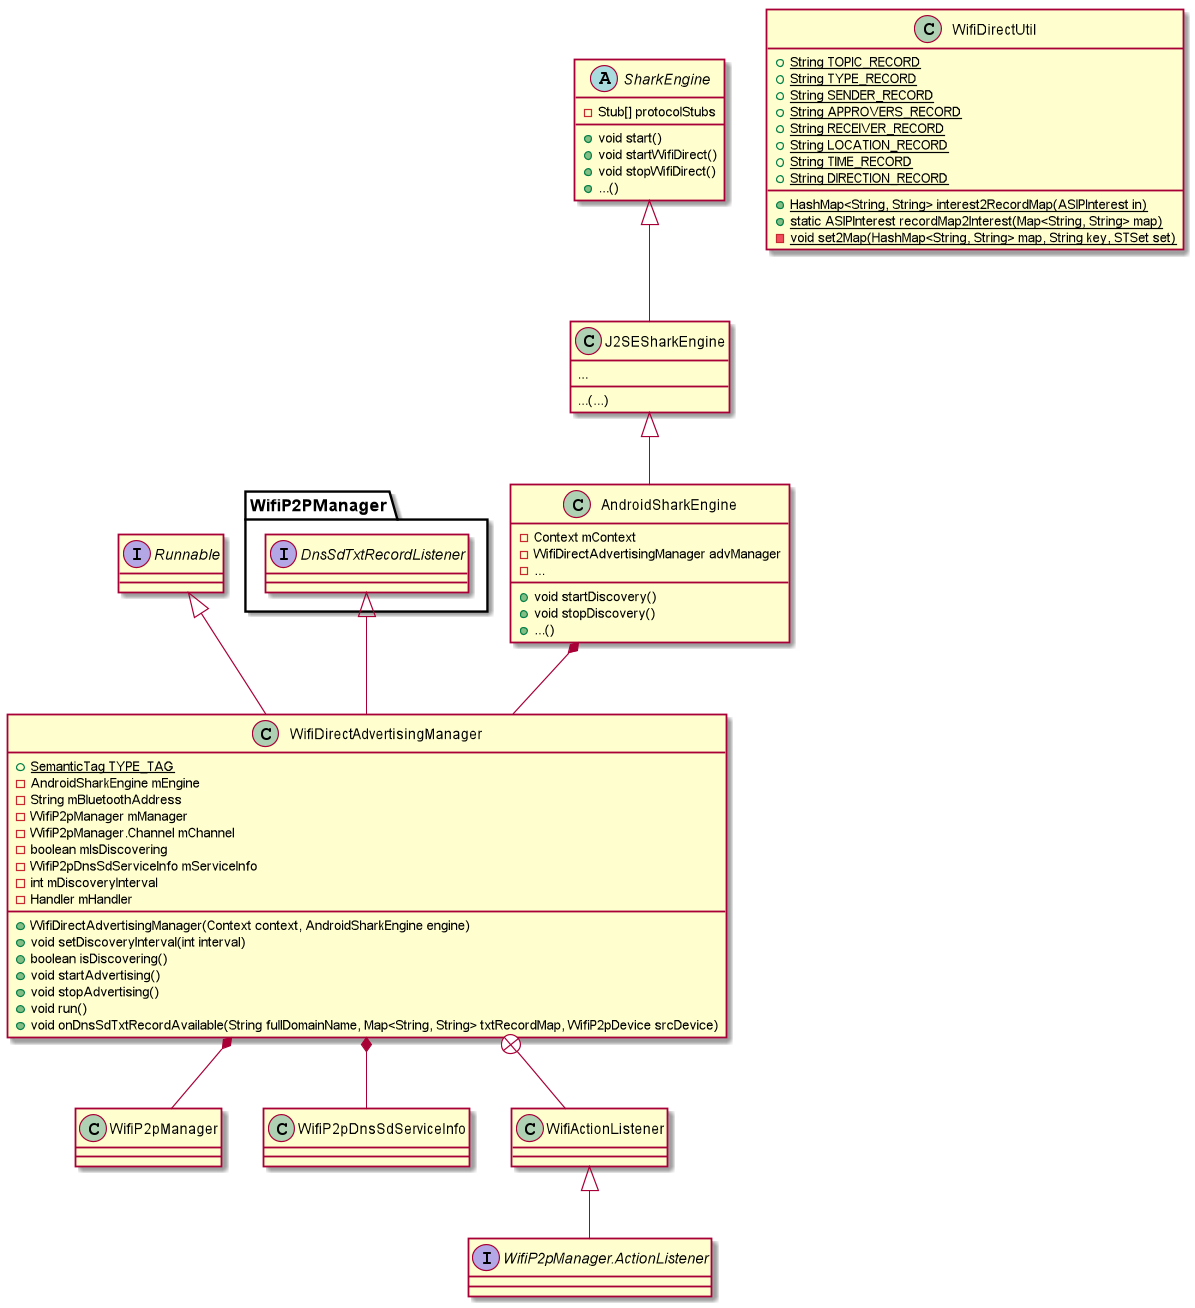
\includegraphics[width=1.1\linewidth]{wifi/images/wifiDirectGesamt.png}}%
	\caption{Die WifiDirect Klassen im Überblick}
	\label{fig:wifiAll}
\end{figure}

\newpage

In der folgenden Grafik sind alle Bestandteile der Radar Komponente abgebildet.
\begin{figure}[H]
	\centering
	\hspace*{1cm}
	\makebox[\linewidth][c]{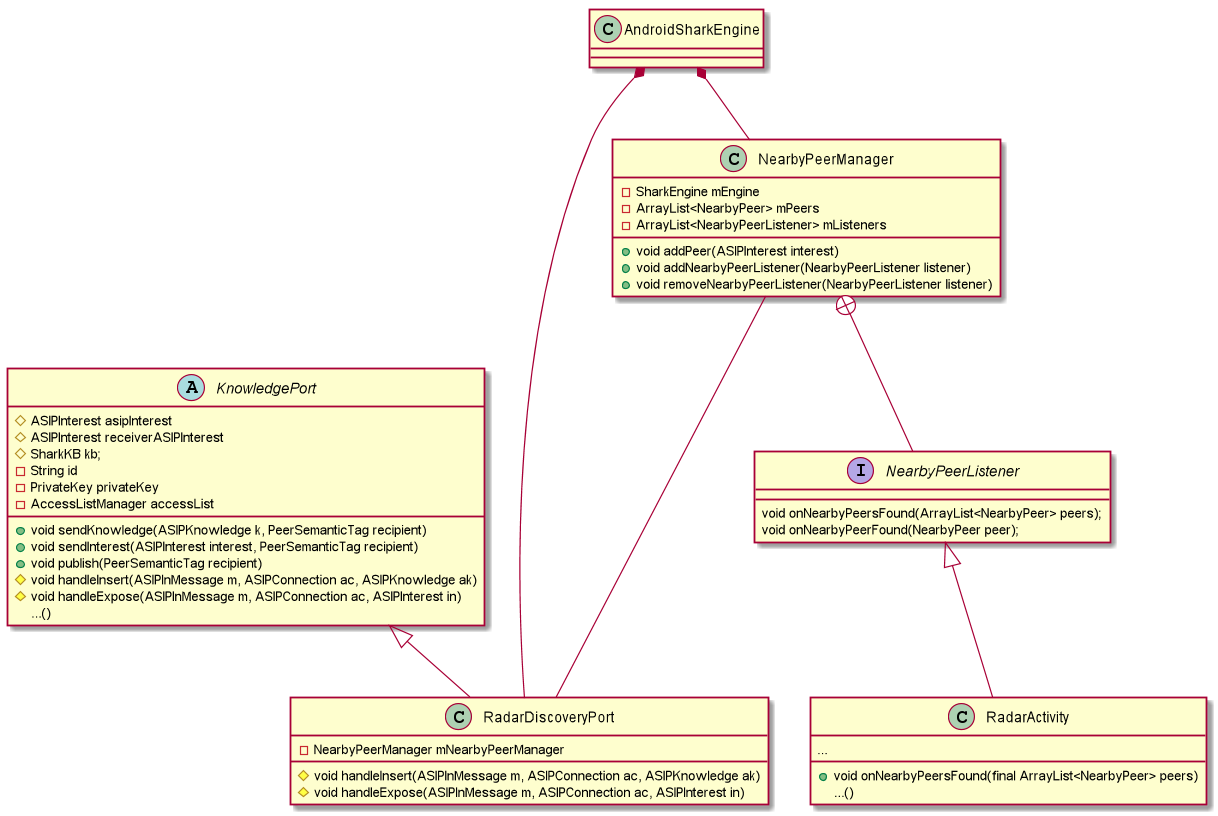
\includegraphics[width=1.1\linewidth]{bluetooth/images/radar.png}}%
	\caption{Die Radar Klassen im Überblick}
	\label{fig:radarAll}
\end{figure}

\newpage

Im folgenden Aktivitätsdiagramm wird das Versenden von Nachrichten per Broadcast abgebildet
\begin{figure}[H]
	\centering
	\hspace*{1cm}
	\makebox[\linewidth][c]{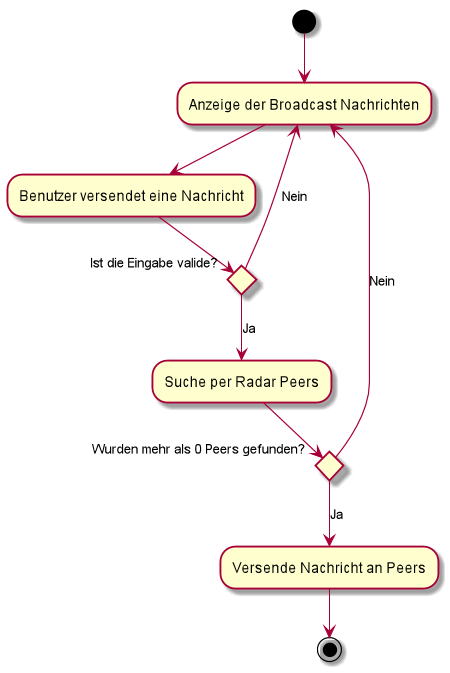
\includegraphics[width=0.5\linewidth]{broadcast/images/broadcastSend.png}}%
	\caption{Versenden von Nachrichten per Broadcast in SharkNet}
	\label{fig:broadcastSend}
\end{figure}

\newpage

Im folgenden Aktivitätsdiagramm wird das Empfangen von Nachrichten per Broadcast abgebildet
\begin{figure}[H]
	\centering
	\hspace*{1cm}
	\makebox[\linewidth][c]{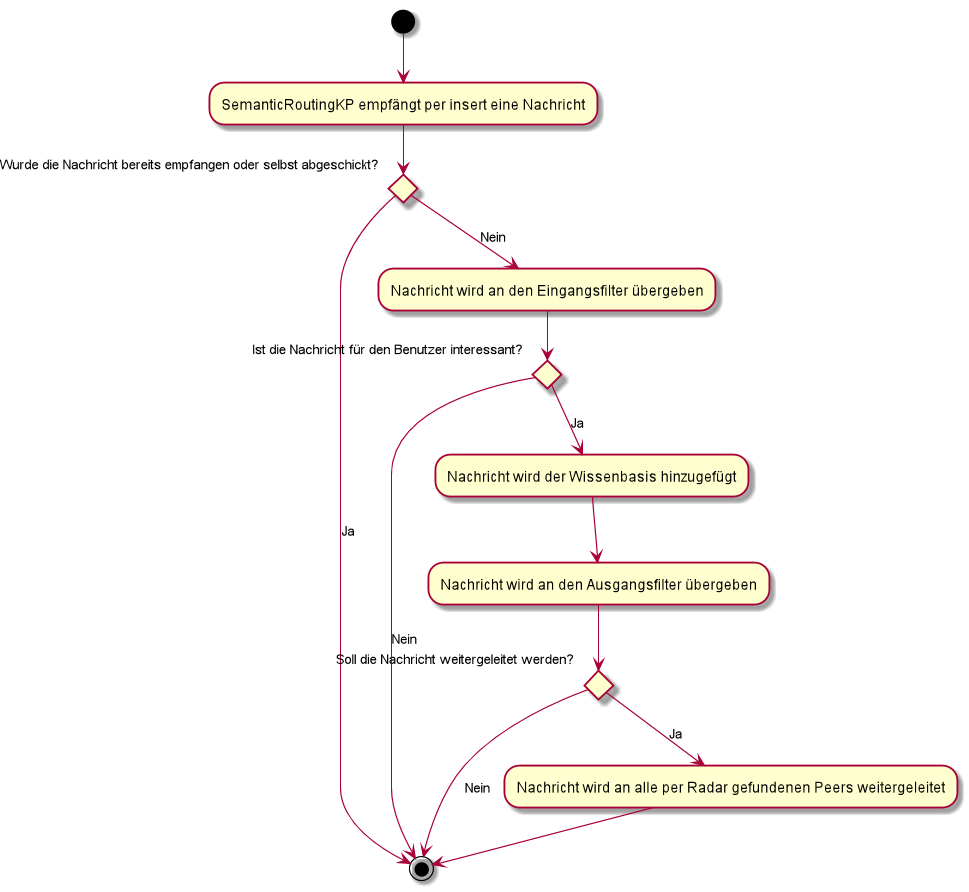
\includegraphics[width=0.9\linewidth]{broadcast/images/broadcastReceive.png}}%
	\caption{Empfangen von Nachrichten per Broadcast in SharkNet}
	\label{fig:broadcastReceive}
\end{figure}

\newpage

Im folgenden Aktivitätsdiagramm wird Filterung von Nachrichten per Eingangsfilter abgebildet
\begin{figure}[H]
	\centering
	\hspace*{1cm}
	\makebox[\linewidth][c]{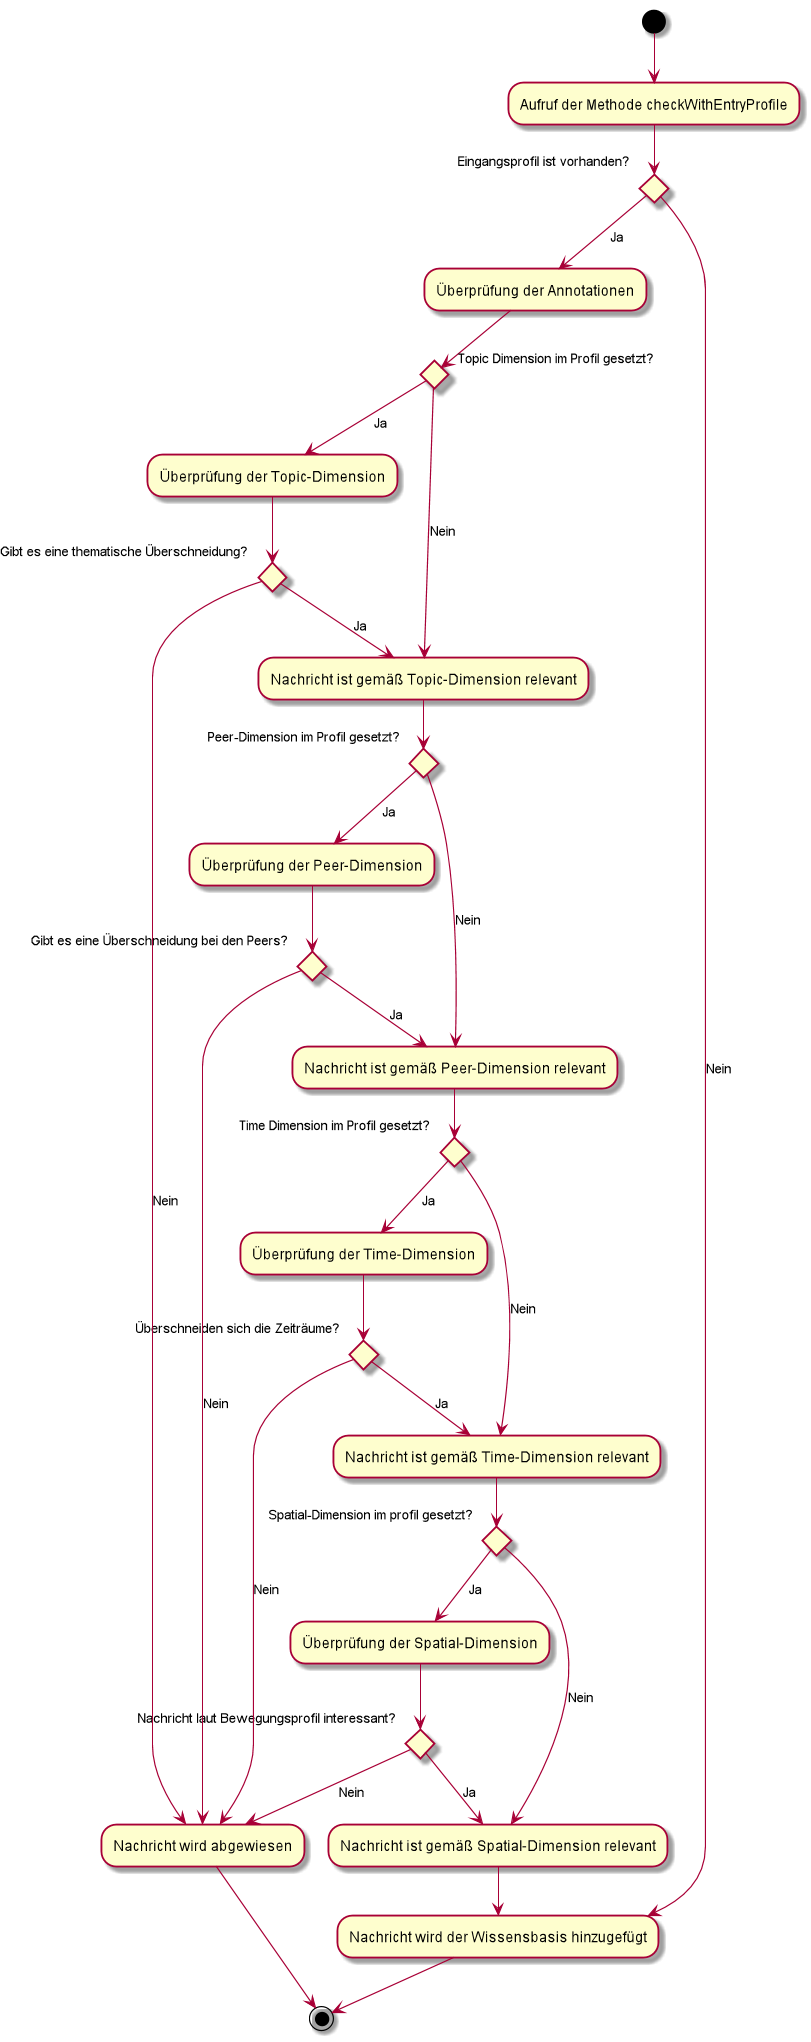
\includegraphics[width=0.6\linewidth]{broadcast/images/entryFilter.png}}%
	\caption{Filterung von Nachrichten per Eingangsfilter in SharkNet}
	\label{fig:entryFilter}
\end{figure}

\newpage

\begin{figure}[H]
	\centering
	\hspace*{1cm}
	\makebox[\linewidth][c]{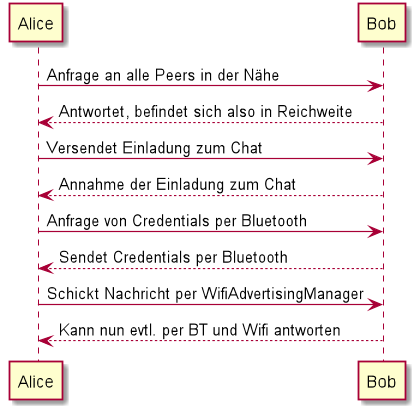
\includegraphics[width=0.7\linewidth]{broadcast/images/communication.png}}%
	\caption{Kommunikation per Chat}
	\label{fig:communication}
\end{figure}

\newpage



\end{document}